%%%%%%%%%%%%%%%%%%%%%%%%%%%%%%%%%%%%%%%%%%%%%%%%%%%%%%%%%%%%%%%%%%%%%%%%%%%%%%%%
% Section 2
\section{Succint Data Structures}

\begin{frame}
\frametitle{Succint data structures}
A succint space data structure 
\begin{itemize}
	\item stores combinatorial objects using space asymptotical equal to the information theoretic lower bound.
	\item supports operations on its elements in $\mathcal{O}$(1) time.
\end{itemize}
\medskip
Note that if the input is taken from a set of $\mathcal{L}$ distinct combinatorial objects then its information-theoretic lower bound is $\lceil log\ \mathcal{L}\rceil $ bits.
\end{frame}

\begin{frame}
\frametitle{Simple lower bounds}
\underline{Example 1}: \textbf{n elements sets} $\mathcal{S} \subseteq \{1, 2, .., n\}$:
\[ log\ 2^n = n\ bits \]

\medskip

\underline{Example 2}: \textbf{length-n strings}:
\[ n\ log\ \sigma\ bits\ (where\ \sigma\ is\ the\ alphabet\ size) \]

\underline{Example 3}: \textbf{n nodes ordered trees}
\[ log\ \frac{1}{2n-1} \binom{2n-1}{n-1} = 2n - \Theta(log\ n) \]
\end{frame}


\begin{frame}
\frametitle{Some insights}
For any data kind there exists a succint representation 
\begin{itemize}
	\item simply obtained by enumerating and assign codes to every possible objects.
	\item that can be represented in $\lceil log\ \mathcal{L} \rceil$ bits
\end{itemize}
Unluckily not every representation is fine.\\
We need compressed structures upon we can implement fast operations.
\end{frame}

\begin{frame}
\frametitle{Rank / Select queries}
Rank and select are the bread and butter of succinct data structures.
\\
Infact almost every operation on these structures can be implemented combining rank and select queries.
\medskip
\begin{itemize}
\item $\mathbf{rank_c(i)}$   = \#occurences of \textbf{c} in the range [0,i]
\item $\mathbf{select_c(i)}$ = position of the i-th occurrence of \textbf{c}. 
\end{itemize}
\begin{figure}
	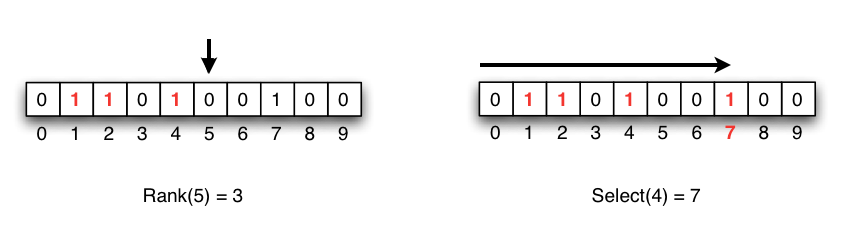
\includegraphics[scale=0.33]{img/ranksel.png}
\end{figure}
\end{frame}


\begin{frame}
\frametitle{Rank / Select queries - Continued}
Speaking of patterns of use, it may also help to keep in mind:
\begin{itemize}
	\item rank is for \textbf{counting}; \\
	two rank queries can count over a range.
	\item select is for \textbf{searching}; \\
	two select queries can find a range
\end{itemize}
\begin{figure}
	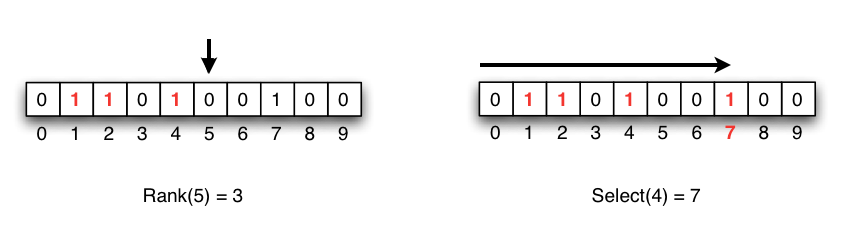
\includegraphics[scale=0.33]{img/ranksel.png}
\end{figure}
\end{frame}


\begin{frame}
\frametitle{Rank / Select queries - Performances}
\begin{itemize}
	\item Assuming that our alphabet size is $ \sigma = polylog(N)$
	ranks and selects can both be done in $\mathcal{O}$(1) time
	by building over our bitvectors simple \textbf{RRR} structures. These additional structures requires just logarithmic space!
	\item for larger alphabets we could use wavelet trees achieving $\mathcal{O}(log \ \sigma)$. Even in this case by using huffman-shaped wavelet trees we can achieve sublinear space usage.
\end{itemize} 
\end{frame}
